% Coupled position projection (contact_projection.py)
\begin{figure}[htbp]
    \centering
    \subfloat[Ball pinched against a wall.]{%
    \begin{tikzpicture}[scale=1]
        \def\r{0.85}\def\h{1.1}
        \fill[wall] (0,-1.6) rectangle (0.3,1.6);
        \draw[thick] (0,-1.6) -- (0,1.6);
        \draw[robotbody] (-2.45-\h,-\h) rectangle (-2.45+\h,\h);
        \draw[ballbody, fill opacity=0.6] (-\r,0) circle (\r);
        \fill (-\r,0) circle (1.3pt);
        \draw[nimp, densely dashed] (-\r,0.25) -- ++(0.5,0);
        \node[red!70!black, font=\scriptsize, align=center] at (-1.9,1.3) {ball: $\tfrac12\delta$, clipped to $0$};
        \draw[vel] (-2.45,0) -- ++(-0.9,0);
        \node[font=\scriptsize, align=center] at (-2.9,-1.45) {robot absorbs $\delta$};
        \draw[{Stealth[length=1.4mm]}-{Stealth[length=1.4mm]}] (-1.7,-0.5) -- (-1.35,-0.5);
        \node[font=\scriptsize, below] at (-1.52,-0.5) {$\delta$};
    \end{tikzpicture}}%
    \hfill
    \subfloat[Five rounds of three disjoint robot pairs.]{%
    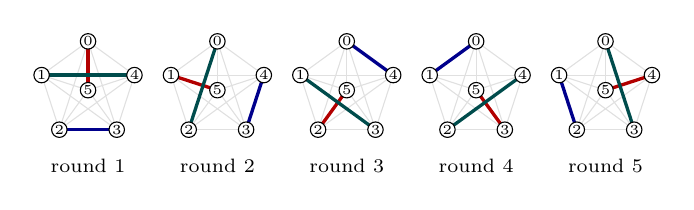
\begin{tikzpicture}[scale=0.62]
        \foreach \k in {0,...,4}{
            \begin{scope}[shift={(\k*2.65,0)}]
                \foreach \i in {0,...,4}
                    \coordinate (n\i) at (90+72*\i:1);
                \coordinate (n5) at (0,0);
                \pgfmathtruncatemacro{\aa}{mod(\k+1,5)}
                \pgfmathtruncatemacro{\ab}{mod(\k+4,5)}
                \pgfmathtruncatemacro{\ba}{mod(\k+2,5)}
                \pgfmathtruncatemacro{\bb}{mod(\k+3,5)}
                \foreach \i in {0,...,4}{\foreach \j in {0,...,5}{\ifnum\i<\j \draw[black!12] (n\i) -- (n\j);\fi}}
                \draw[very thick, red!70!black] (n\k) -- (n5);
                \draw[very thick, teal!60!black] (n\aa) -- (n\ab);
                \draw[very thick, blue!55!black] (n\ba) -- (n\bb);
                \foreach \i in {0,...,5}
                    \fill[white] (n\i) circle (4.5pt);
                \foreach \i in {0,...,5}{
                    \draw (n\i) circle (4.5pt);
                    \node[font=\tiny] at (n\i) {\i};
                }
                \node[font=\scriptsize] at (0,-1.55) {round \the\numexpr\k+1\relax};
            \end{scope}
        }
    \end{tikzpicture}}
    \caption{Position-only projection.  (a)~Each overlap is split evenly, but a ball
    correction is clipped at the first static wall and the robot takes the remainder;
    likewise a robot that the field clamp moved is pinned in the next iteration.
    (b)~The 15 robot pairs are relaxed as five perfect matchings of the six robots,
    so each round corrects three independent pairs in parallel before re-clamping
    to the field.}
    \label{fig:projection}
\end{figure}
